% Options for packages loaded elsewhere
\PassOptionsToPackage{unicode}{hyperref}
\PassOptionsToPackage{hyphens}{url}
\PassOptionsToPackage{dvipsnames,svgnames,x11names}{xcolor}
%
\documentclass[
  letterpaper,
  DIV=11,
  numbers=noendperiod]{scrartcl}

\usepackage{amsmath,amssymb}
\usepackage{lmodern}
\usepackage{iftex}
\ifPDFTeX
  \usepackage[T1]{fontenc}
  \usepackage[utf8]{inputenc}
  \usepackage{textcomp} % provide euro and other symbols
\else % if luatex or xetex
  \usepackage{unicode-math}
  \defaultfontfeatures{Scale=MatchLowercase}
  \defaultfontfeatures[\rmfamily]{Ligatures=TeX,Scale=1}
\fi
% Use upquote if available, for straight quotes in verbatim environments
\IfFileExists{upquote.sty}{\usepackage{upquote}}{}
\IfFileExists{microtype.sty}{% use microtype if available
  \usepackage[]{microtype}
  \UseMicrotypeSet[protrusion]{basicmath} % disable protrusion for tt fonts
}{}
\makeatletter
\@ifundefined{KOMAClassName}{% if non-KOMA class
  \IfFileExists{parskip.sty}{%
    \usepackage{parskip}
  }{% else
    \setlength{\parindent}{0pt}
    \setlength{\parskip}{6pt plus 2pt minus 1pt}}
}{% if KOMA class
  \KOMAoptions{parskip=half}}
\makeatother
\usepackage{xcolor}
\setlength{\emergencystretch}{3em} % prevent overfull lines
\setcounter{secnumdepth}{2}
% Make \paragraph and \subparagraph free-standing
\ifx\paragraph\undefined\else
  \let\oldparagraph\paragraph
  \renewcommand{\paragraph}[1]{\oldparagraph{#1}\mbox{}}
\fi
\ifx\subparagraph\undefined\else
  \let\oldsubparagraph\subparagraph
  \renewcommand{\subparagraph}[1]{\oldsubparagraph{#1}\mbox{}}
\fi


\providecommand{\tightlist}{%
  \setlength{\itemsep}{0pt}\setlength{\parskip}{0pt}}\usepackage{longtable,booktabs,array}
\usepackage{calc} % for calculating minipage widths
% Correct order of tables after \paragraph or \subparagraph
\usepackage{etoolbox}
\makeatletter
\patchcmd\longtable{\par}{\if@noskipsec\mbox{}\fi\par}{}{}
\makeatother
% Allow footnotes in longtable head/foot
\IfFileExists{footnotehyper.sty}{\usepackage{footnotehyper}}{\usepackage{footnote}}
\makesavenoteenv{longtable}
\usepackage{graphicx}
\makeatletter
\def\maxwidth{\ifdim\Gin@nat@width>\linewidth\linewidth\else\Gin@nat@width\fi}
\def\maxheight{\ifdim\Gin@nat@height>\textheight\textheight\else\Gin@nat@height\fi}
\makeatother
% Scale images if necessary, so that they will not overflow the page
% margins by default, and it is still possible to overwrite the defaults
% using explicit options in \includegraphics[width, height, ...]{}
\setkeys{Gin}{width=\maxwidth,height=\maxheight,keepaspectratio}
% Set default figure placement to htbp
\makeatletter
\def\fps@figure{htbp}
\makeatother

\KOMAoption{captions}{tableheading}
\makeatletter
\makeatother
\makeatletter
\makeatother
\makeatletter
\@ifpackageloaded{caption}{}{\usepackage{caption}}
\AtBeginDocument{%
\ifdefined\contentsname
  \renewcommand*\contentsname{Table of contents}
\else
  \newcommand\contentsname{Table of contents}
\fi
\ifdefined\listfigurename
  \renewcommand*\listfigurename{List of Figures}
\else
  \newcommand\listfigurename{List of Figures}
\fi
\ifdefined\listtablename
  \renewcommand*\listtablename{List of Tables}
\else
  \newcommand\listtablename{List of Tables}
\fi
\ifdefined\figurename
  \renewcommand*\figurename{Figure}
\else
  \newcommand\figurename{Figure}
\fi
\ifdefined\tablename
  \renewcommand*\tablename{Table}
\else
  \newcommand\tablename{Table}
\fi
}
\@ifpackageloaded{float}{}{\usepackage{float}}
\floatstyle{ruled}
\@ifundefined{c@chapter}{\newfloat{codelisting}{h}{lop}}{\newfloat{codelisting}{h}{lop}[chapter]}
\floatname{codelisting}{Listing}
\newcommand*\listoflistings{\listof{codelisting}{List of Listings}}
\makeatother
\makeatletter
\@ifpackageloaded{caption}{}{\usepackage{caption}}
\@ifpackageloaded{subcaption}{}{\usepackage{subcaption}}
\makeatother
\makeatletter
\@ifpackageloaded{tcolorbox}{}{\usepackage[many]{tcolorbox}}
\makeatother
\makeatletter
\@ifundefined{shadecolor}{\definecolor{shadecolor}{rgb}{.97, .97, .97}}
\makeatother
\makeatletter
\makeatother
\ifLuaTeX
  \usepackage{selnolig}  % disable illegal ligatures
\fi
\IfFileExists{bookmark.sty}{\usepackage{bookmark}}{\usepackage{hyperref}}
\IfFileExists{xurl.sty}{\usepackage{xurl}}{} % add URL line breaks if available
\urlstyle{same} % disable monospaced font for URLs
\hypersetup{
  pdftitle={HIMYM},
  pdfauthor={Aziz Aliev},
  colorlinks=true,
  linkcolor={blue},
  filecolor={Maroon},
  citecolor={Blue},
  urlcolor={Blue},
  pdfcreator={LaTeX via pandoc}}

\title{HIMYM}
\author{Aziz Aliev}
\date{4/20/23}

\begin{document}
\maketitle
\ifdefined\Shaded\renewenvironment{Shaded}{\begin{tcolorbox}[breakable, borderline west={3pt}{0pt}{shadecolor}, interior hidden, frame hidden, enhanced, sharp corners, boxrule=0pt]}{\end{tcolorbox}}\fi

\listoffigures
\listoftables
\hypertarget{how-i-met-your-mother}{%
\section{\texorpdfstring{\emph{How I Met Your
Mother}}{How I Met Your Mother}}\label{how-i-met-your-mother}}

\hypertarget{brief-description}{%
\subsection{Brief Description}\label{brief-description}}

``How I Met Your Mother'' (often abbreviated as HIMYM) is an American
sitcom, created by Craig Thomas and Carter Bays for CBS. The series,
which aired from September 19, 2005, to March 31, 2014, follows the main
character, Ted Mosby, and his group of friends in New York City's
Manhattan. As a framing device, Ted, in 2030, recounts to his son, Luke,
and daughter, Penny, the events from September 2005 to May 2013 that led
him to meet their mother. ``How I Met Your Mother'' is a joint
production by Bays \& Thomas Productions and 20th Century Fox Television
and syndicated by 20th Television (now Disney-ABC Domestic Television).

The series was loosely inspired by Thomas and Bays' friendship when they
both lived in New York. The vast majority of episodes were directed by
Pamela Fryman, who directed 196 episodes out of 208. The other directors
were Rob Greenberg (7 episodes), Michael Shea (4 episodes), and Neil
Patrick Harris (1 episode).

Known for its unique structure, humor, and incorporation of dramatic
elements, ``How I Met Your Mother'' was popular throughout its run. It
initially received positive reviews upon release, but reception became
more mixed as the seasons went on. The show was nominated for 91 awards
and received 21. In 2010, Alyson Hannigan won the People's Choice Award
for Favorite TV Comedy Actress. In 2012, seven years after its premiere,
the series won the People's Choice Award for Favorite Network TV Comedy,
and Neil Patrick Harris won the award for Favorite TV Comedy Actor
twice.

\begin{figure}

{\centering 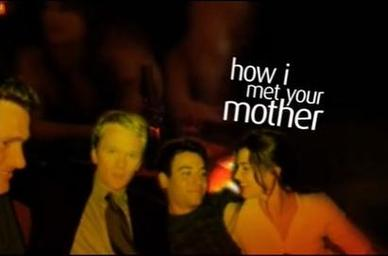
\includegraphics{Howimetyourmother.jpg}

}

\caption{\textbf{A photo from the series}}

\end{figure}

\hypertarget{basic-statistics-for-how-i-met-your-mother-himym}{%
\section{Basic Statistics for How I Met Your Mother
(HIMYM)}\label{basic-statistics-for-how-i-met-your-mother-himym}}

Here are some basic statistics for the TV show ``How I Met Your
Mother'':

\begin{itemize}
\tightlist
\item
  Total number of seasons: 9
\item
  Total number of episodes: 208
\item
  Average episode length: 22 minutes
\item
  Total runtime: 91 hours and 16 minutes
\item
  First episode air date: September 19, 2005
\item
  Last episode air date: March 31, 2014
\end{itemize}

\hypertarget{ratings}{%
\subsection{Ratings}\label{ratings}}

\begin{itemize}
\tightlist
\item
  IMDb rating: 8.3/10
\item
  Rotten Tomatoes score: 83\%
\item
  Metacritic score: 69/100
\end{itemize}

\hypertarget{awards}{%
\subsection{Awards}\label{awards}}

\begin{itemize}
\tightlist
\item
  Primetime Emmy Awards: 10 wins and 72 nominations
\item
  People's Choice Awards: 8 wins and 21 nominations
\item
  Golden Globe Awards: 2 nominations
\end{itemize}

\hypertarget{a-graph-of-the-viewership-over-time}{%
\section{A graph of the viewership over
time}\label{a-graph-of-the-viewership-over-time}}

\hypertarget{code-block}{%
\subsubsection{code block}\label{code-block}}

\textbf{Load necessary packages}

library(tidyverse)

\textbf{Create a data frame with viewership data}

himym \textless- data.frame( year = c(2005, 2006, 2007, 2008, 2009,
2010, 2011, 2012, 2013, 2014), viewers = c(10.94, 9.71, 8.68, 9.35,
9.14, 9.11, 8.45, 8.01, 7.48, 12.94) )

\textbf{Create a plot with the x-axis showing only integers}

ggplot(himym, aes(x = year, y = viewers)) + geom\_line() +
scale\_x\_continuous(breaks = himym\$year, expand = c(0,0)) + labs(x =
``Year'', y = ``Viewers (millions)'', title = ``Viewership of How I Met
Your Mother'')

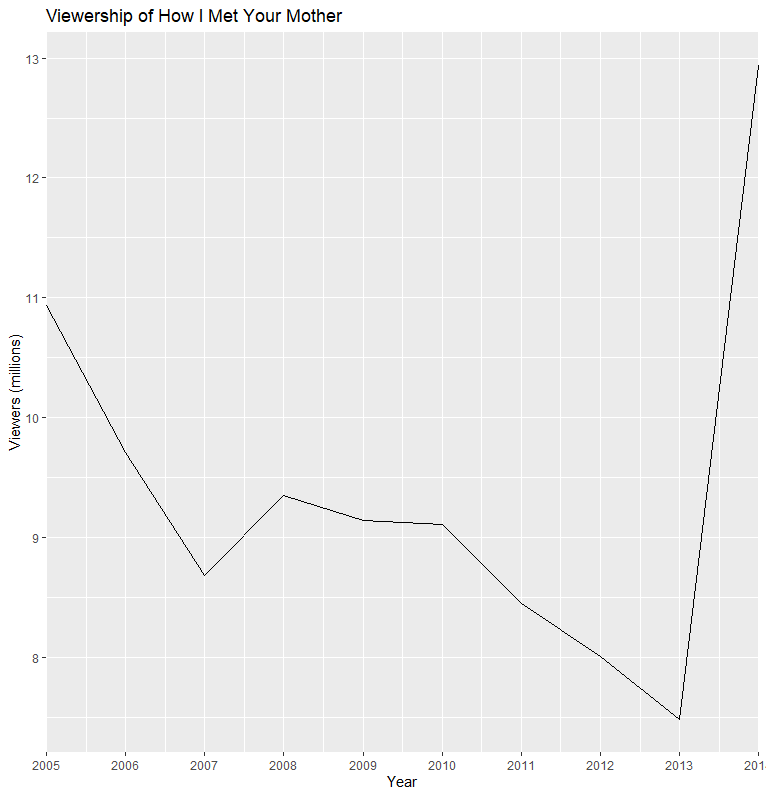
\includegraphics{Rplot.png}

\hypertarget{a-graph-of-the-episode-to-episode-or-season-to-season-changes-ratings}{%
\section{A graph of the episode-to-episode (or season-to-season) changes
ratings}\label{a-graph-of-the-episode-to-episode-or-season-to-season-changes-ratings}}

\textbf{Create a data frame with the season-to-season viewership data}

viewership \textless- data.frame( season = 1:9, viewers = c(10.94, 9.47,
8.43, 8.59, 9.01, 8.24, 7.98, 7.88, 7.37) )

\textbf{Create a line graph using ggplot2}

library(ggplot2)

ggplot(viewership, aes(x = season, y = viewers)) + geom\_line() +
geom\_point() + labs(title = ``Season-to-Season Changes in HIMYM
Viewership'', x = ``Season'', y = ``Average Viewers (in millions)'')

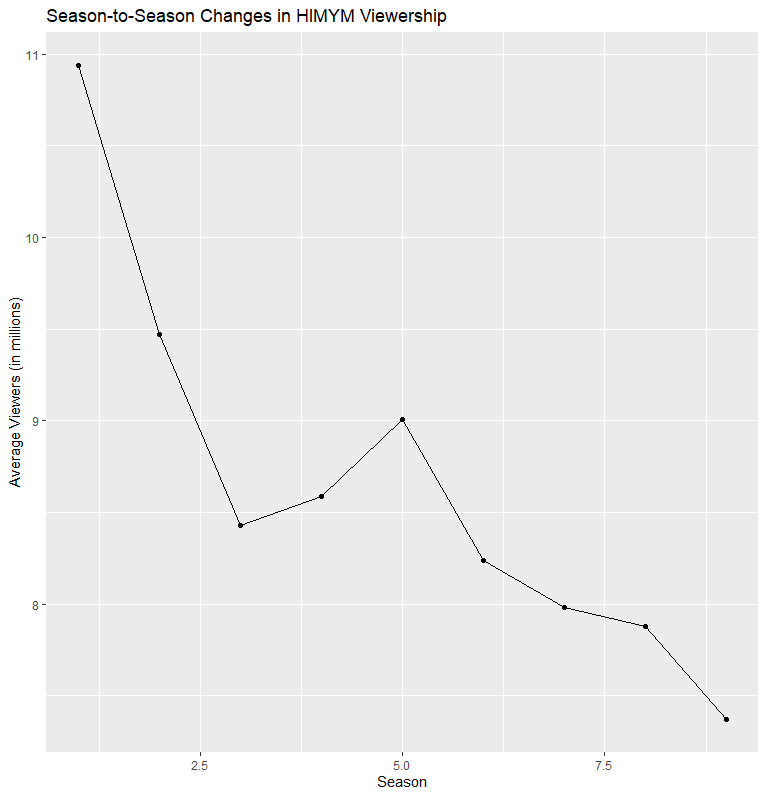
\includegraphics{Rplot01.png}



\end{document}
